\chapter{Introduction}
\Atlas is an ECMWF software framework for parallel flexible 
data-structures supporting structured/unstructured grids, 
structured/unstructured meshes, various function spaces 
and utilities.  
The main aim of \Atlas is to investigate and develop more 
scalable dynamical core options for numerical weather prediction 
(NWP). \Atlas is also intended to create modern interpolation 
and product generation software.

\Atlas is predominantly written in C++, with the main features 
available to Fortran through an F2003 interface. To be used 
effectively, it requires some knowledge of Unix (such as Linux). 
It is known to run on a number of systems, some of which are 
directly supported by ECMWF.

\Atlas includes the following macro data objects.
%
\begin{itemize}
\item Grid: a list of coordinates (i.e. points) without connectivity rules;
\item Mesh: a collection of elements linked by precise connectivity rules;
\item Field: a physical quantity such as wind velocity or pressure;
\item FieldSet: a collection of Fields;
\item FunctionSpace: a given spatial discretization space (e.g. spectral, 
finite element, etc.).
\end{itemize}
%
From these objects it is possible to construct new algorithms 
to be tested within the context of numerical weather prediction 
(NWP), to generate and manipulate grids for production 
cases, etc. The overall structure of the library is depicted 
in \fig{fig:intro-schematics}.

From this figure, we note that there is the additional object 
called Metadata and related to the Field object. Metadata 
contains a description of a given Field (e.g. units, etc.).
We also note that the Mesh object is formed by the Nodes 
and HybridElements objects, with the last being composed 
by Elements. These additional items represents the bricks 
to ultimately build the mesh object.
 
The structure in Fig. \ref{fig:intro-schematics} will be 
further explained in chapter \ref{chap:structure}.
%
\begin{figure}[htb!]
\centering
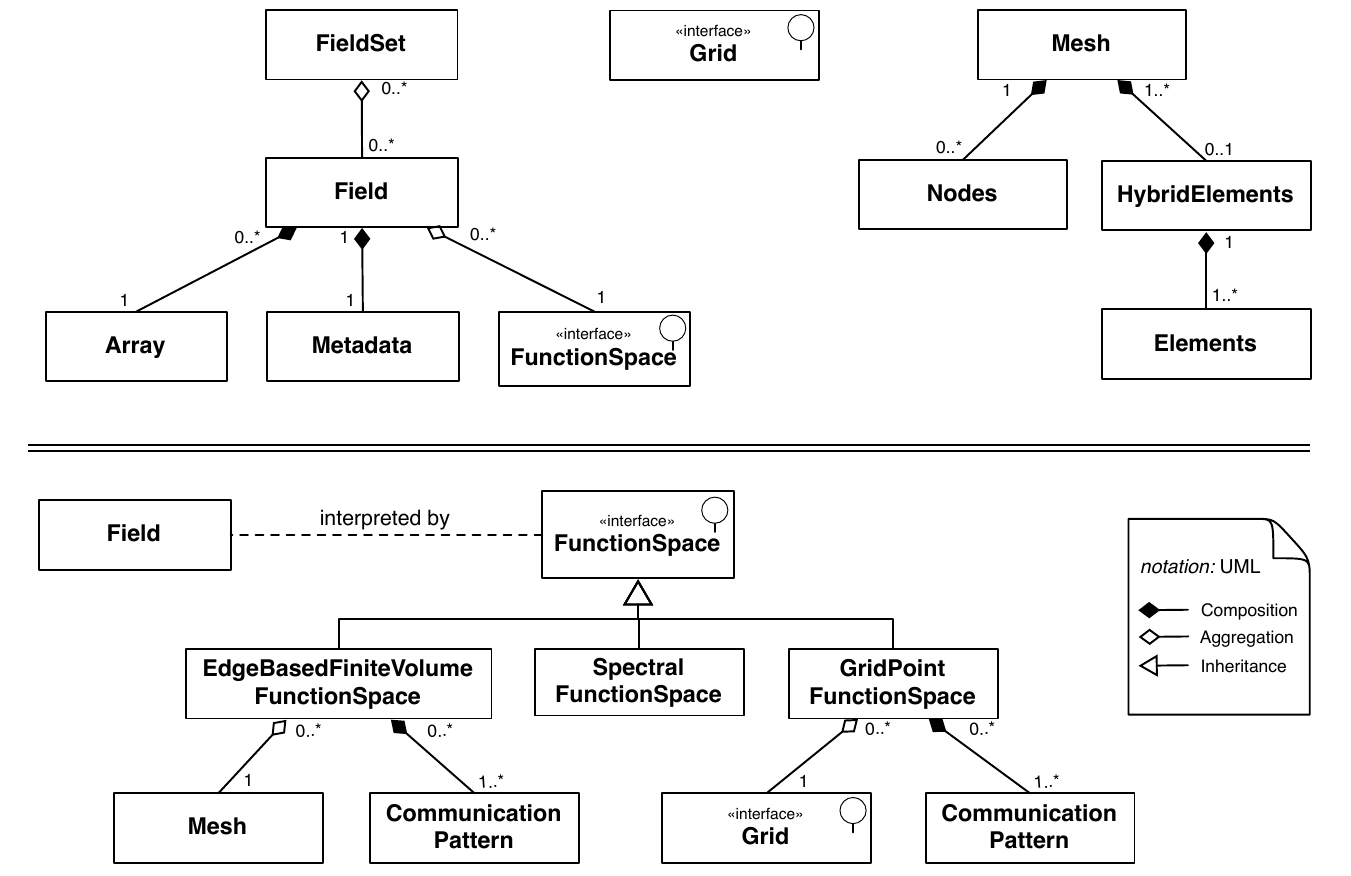
\includegraphics[width=0.95\textwidth]{imgs/schematics.png}
\caption{Schematics of the \Atlas library.}
\label{fig:intro-schematics}
\end{figure}
%